% =============================================================================
% Appendix J: ESP32 Firmware Source Code
% =============================================================================

\subsection{ESP32 Firmware Source Code}\label{app:firmware-code}

This appendix contains the complete source code for the STAR ESP32 firmware framework. The firmware implements a production-ready embedded system with dependency injection, thread-safe communication, and comprehensive error handling. The full repository with all libraries is available at the project GitHub.

% -----------------------------------------------------------------------------
\subsubsection{Dependency Inversion Principle (DIP) in Embedded C}
% -----------------------------------------------------------------------------

The STAR firmware implements the \textbf{Dependency Inversion Principle (DIP)}, the ``D'' in SOLID, in pure C without object-oriented language features. DIP states:

\begin{enumerate}
    \item \textbf{High-level modules should not depend on low-level modules.} Both should depend on abstractions.
    \item \textbf{Abstractions should not depend on details.} Details should depend on abstractions.
\end{enumerate}

In traditional embedded C, sensor drivers often directly call I\textsuperscript{2}C or SPI functions, creating tight coupling that makes testing and hardware changes difficult. DIP inverts this relationship:

\begin{figure}[H]
\centering
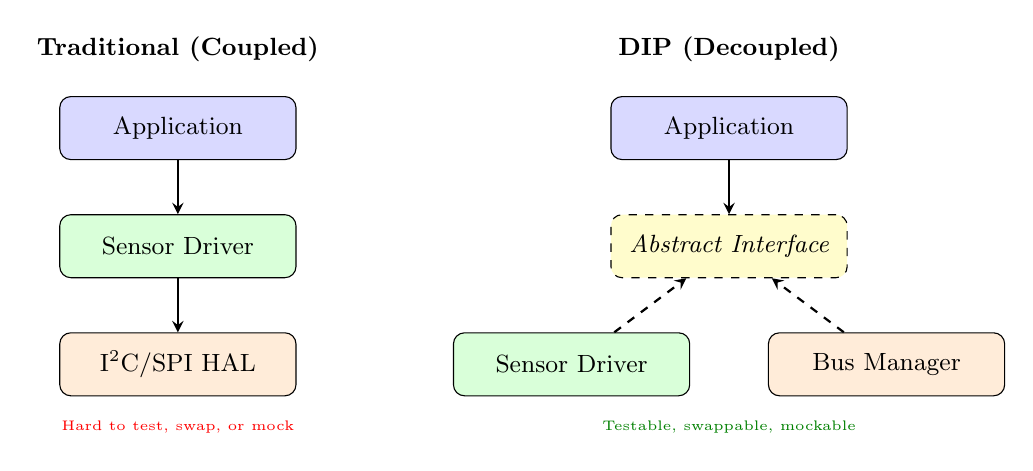
\begin{tikzpicture}[
    node distance=1cm and 2cm,
    block/.style={rectangle, draw, rounded corners, minimum width=3cm, minimum height=0.8cm, align=center, font=\small},
    iface/.style={rectangle, draw, rounded corners, dashed, minimum width=3cm, minimum height=0.8cm, align=center, font=\small\itshape},
    arrow/.style={->, thick, >=stealth}
]
    % Traditional (left side)
    \node[font=\small\bfseries] at (-3.5, 2.5) {Traditional (Coupled)};
    \node[block, fill=blue!15] (app1) at (-3.5, 1.5) {Application};
    \node[block, fill=green!15] (driver1) at (-3.5, 0) {Sensor Driver};
    \node[block, fill=orange!15] (hw1) at (-3.5, -1.5) {I\textsuperscript{2}C/SPI HAL};
    \draw[arrow] (app1) -- (driver1);
    \draw[arrow] (driver1) -- (hw1);
    \node[font=\tiny, red] at (-3.5, -2.3) {Hard to test, swap, or mock};

    % DIP (right side)
    \node[font=\small\bfseries] at (3.5, 2.5) {DIP (Decoupled)};
    \node[block, fill=blue!15] (app2) at (3.5, 1.5) {Application};
    \node[iface, fill=yellow!20] (iface) at (3.5, 0) {Abstract Interface};
    \node[block, fill=green!15] (driver2) at (1.5, -1.5) {Sensor Driver};
    \node[block, fill=orange!15] (hw2) at (5.5, -1.5) {Bus Manager};
    \draw[arrow] (app2) -- (iface);
    \draw[arrow, dashed] (driver2) -- (iface);
    \draw[arrow, dashed] (hw2) -- (iface);
    \node[font=\tiny, green!50!black] at (3.5, -2.3) {Testable, swappable, mockable};
\end{tikzpicture}
\caption{Traditional vs. DIP Architecture Comparison}
\label{fig:dip-comparison}
\end{figure}

\paragraph{Implementation in C.}
DIP is implemented using \texttt{struct}s with function pointers. Each interface defines a contract that implementations must fulfill:

\begin{lstlisting}[language=C, caption={Abstract Interface Definition}, basicstyle=\tiny\ttfamily, frame=single, numbers=left, float=h]
/* star_error_interface.h - Abstract contract for error handling */
typedef struct star_error_interface {
    /* Function pointers define the contract */
    esp_err_t (*record_error)(void* ctx, esp_err_t error, const char* message,
                              const char* file, int line, const char* func);
    bool (*can_retry)(void* ctx);
    esp_err_t (*reset_state)(void* ctx);

    /* Opaque pointer to concrete implementation - could be ANY error handler */
    void* ctx;
} star_error_interface_t;
\end{lstlisting}

Concrete implementations provide the actual behavior:

\begin{lstlisting}[language=C, caption={Concrete Implementation Binding}, basicstyle=\tiny\ttfamily, frame=single, numbers=left, float=h]
/* star_error_handler.c - Concrete implementation with retry logic */
void error_handler_get_interface(star_error_interface_t* iface,
                                  error_handler_t* handler) {
    /* Bind function pointers to concrete implementation */
    iface->record_error = internal_record_error;
    iface->can_retry    = internal_can_retry;
    iface->reset_state  = internal_reset_state;
    iface->ctx          = handler;  /* Pass concrete instance */
}
\end{lstlisting}

Components receive interfaces via constructor injection:

\begin{lstlisting}[language=C, caption={Dependency Injection via Constructor}, basicstyle=\tiny\ttfamily, frame=single, numbers=left, float=h]
/* Sensor driver receives abstract interfaces, not concrete implementations */
esp_err_t star_sensor_hcsr04_init(hcsr04_handle_t* handle,
                                   star_bus_manager_t* manager,  /* Bus abstraction */
                                   const char* bus_name,
                                   star_error_interface_t* error_iface,  /* DIP */
                                   const hcsr04_config_t* config) {
    /* Store interface reference - driver doesn't know the concrete type */
    handle->error_iface = error_iface;

    /* Use interface without knowing implementation details */
    if (error_iface != NULL) {
        STAR_IFACE_RECORD_ERROR(error_iface, ESP_OK, "HC-SR04 initialized");
    }
    return ESP_OK;
}
\end{lstlisting}

\paragraph{Benefits in Practice.}
\begin{itemize}
    \item \textbf{Unit Testing}: Pass mock interfaces that record calls instead of touching hardware
    \item \textbf{Hardware Swapping}: Replace BNO055 with MPU6050 by providing a different implementation of the same interface
    \item \textbf{Optional Features}: Pass \texttt{NULL} for optional interfaces (e.g., error handler) for minimal builds
    \item \textbf{No Circular Dependencies}: Interfaces live in \texttt{star\_core}; implementations depend on interfaces, not vice versa
\end{itemize}

% -----------------------------------------------------------------------------
\subsubsection{System Call Graphs}
% -----------------------------------------------------------------------------

The following call graphs were generated using GNU cflow, Egypt, and Graphviz to visualize the firmware's execution flow and validate the layered architecture. The complete call graph shows all function relationships in the codebase.

\begin{figure}[H]
\centering

\includegraphics[width=\textwidth, height=0.85\textheight, keepaspectratio]{figures/firmware/callgraphs/callgraph_application.pdf}
\caption{Application Layer Call Graph: Entry Point and Task Initialization}
\label{fig:callgraph-application-app}
\end{figure}

% -----------------------------------------------------------------------------
\subsubsection{Main Application (\texttt{main.c})}
% -----------------------------------------------------------------------------

The main application orchestrates system initialization following the dependency injection pattern. It creates abstract interfaces, initializes the bus manager, configures hardware buses, and starts FreeRTOS tasks.

\begin{lstlisting}[language=C, caption={STAR Firmware Main Application (main.c)}, basicstyle=\tiny\ttfamily, frame=single, numbers=left, breaklines=true]
#include <esp_log.h>
#include <freertos/FreeRTOS.h>
#include <freertos/task.h>

#include "include/system_config.h"
#include "modules/include/shared_data.h"
#include "star_bus_config.h"
#include "star_bus_dht22_proprietary.h"
#include "star_bus_gpio.h"
#include "star_bus_manager.h"
#include "star_error_handler.h"
#include "star_error_interface.h"
#include "star_pin_interface.h"
#include "star_pin_validator.h"
#include "star_sensor_pca9685.h"
#include "tasks/include/dht22_task.h"
#include "tasks/include/led_task.h"
#include "tasks/include/sensor_task.h"
#include "tasks/include/watchdog_task.h"

/* Error Handler Configuration for Fast LED Response */
static const uint8_t  s_main_fast_error_retries    = 2;
static const uint32_t s_main_fast_error_base_delay = 10;
static const uint32_t s_main_fast_error_max_delay  = 50;
static const uint32_t s_main_loop_sleep_ms = 10000;

static const char* s_TAG = "MAIN";

static esp_err_t initialize_hardware_buses(star_bus_manager_t* const bus_manager)
{
  esp_err_t ret;

  /* Initialize DHT22 proprietary bus */
  ESP_LOGI(s_TAG, "Setting up DHT22 on GPIO %d", STAR_SYSTEM_CONFIG.gpio.dht22_data);
  star_dht22_config_t dht22_config = STAR_DHT22_CONFIG_DEFAULT();
  dht22_config.gpio_pin            = STAR_SYSTEM_CONFIG.gpio.dht22_data;

  ret = star_bus_dht22_init(bus_manager, STAR_SYSTEM_CONFIG.bus_names.dht22, &dht22_config);
  if (ret != ESP_OK) {
    ESP_LOGE(s_TAG, "Failed to init DHT22: %s", esp_err_to_name(ret));
    return ret;
  }

  /* Initialize GPIO bus for HC-SR04 sensors */
  const gpio_num_t hcsr04_pins[] = {
    STAR_SYSTEM_CONFIG.gpio.left_trig,  STAR_SYSTEM_CONFIG.gpio.left_echo,
    STAR_SYSTEM_CONFIG.gpio.right_trig, STAR_SYSTEM_CONFIG.gpio.right_echo};
  star_bus_config_t* hcsr04_gpio_bus = star_bus_config_create_gpio(
    STAR_SYSTEM_CONFIG.bus_names.hcsr04, hcsr04_pins, 4);

  if (hcsr04_gpio_bus == NULL) {
    ESP_LOGE(s_TAG, "Failed to create GPIO bus for HC-SR04");
    return ESP_ERR_NO_MEM;
  }

  ret = star_bus_manager_add_bus(bus_manager, hcsr04_gpio_bus);
  if (ret != ESP_OK) {
    ESP_LOGE(s_TAG, "Failed to add GPIO bus: %s", esp_err_to_name(ret));
    star_bus_config_destroy(hcsr04_gpio_bus);
    return ret;
  }

  /* Initialize I2C bus for PCA9685 PWM controller */
  star_bus_config_t* pwm_bus = star_bus_config_create_i2c(
    STAR_SYSTEM_CONFIG.bus_names.pca9685,
    STAR_SYSTEM_CONFIG.pca9685.i2c_port,
    STAR_SYSTEM_CONFIG.pca9685.i2c_addr,
    STAR_SYSTEM_CONFIG.gpio.pca9685_sda,
    STAR_SYSTEM_CONFIG.gpio.pca9685_scl,
    STAR_SYSTEM_CONFIG.pca9685.i2c_frequency);

  if (pwm_bus == NULL) {
    ESP_LOGE(s_TAG, "Failed to create I2C bus for PCA9685");
    return ESP_ERR_NO_MEM;
  }

  ret = star_bus_manager_add_bus(bus_manager, pwm_bus);
  if (ret != ESP_OK) {
    ESP_LOGE(s_TAG, "Failed to add I2C bus: %s", esp_err_to_name(ret));
    star_bus_config_destroy(pwm_bus);
    return ret;
  }

  ESP_LOGI(s_TAG, "All hardware buses initialized successfully");
  return ESP_OK;
}

static esp_err_t initialize_pca9685(star_bus_manager_t* const bus_manager,
                                    star_error_interface_t* const error_iface,
                                    pca9685_handle_t* const pca_handle)
{
  const pca9685_config_t pca9685_config = {
    .i2c_addr      = STAR_SYSTEM_CONFIG.pca9685.i2c_addr,
    .pwm_freq      = STAR_SYSTEM_CONFIG.pca9685.pwm_frequency_hz,
    .output_mode   = k_pca9685_output_totem_pole,
    .ext_clock     = false,
    .invert_output = false};

  esp_err_t ret = star_sensor_pca9685_init(
    pca_handle, bus_manager, STAR_SYSTEM_CONFIG.bus_names.pca9685,
    error_iface, STAR_SYSTEM_CONFIG.gpio.pca9685_oe, false, &pca9685_config);

  if (ret != ESP_OK) {
    ESP_LOGE(s_TAG, "Failed to init PCA9685: %s", esp_err_to_name(ret));
    return ret;
  }

  ESP_LOGI(s_TAG, "PCA9685 initialized successfully");
  return ESP_OK;
}

static esp_err_t start_system_tasks(star_bus_manager_t* const bus_manager,
                                    star_error_interface_t* const error_iface,
                                    const pca9685_handle_t* pca_handle)
{
  esp_err_t ret;

  ret = dht22_task_start(bus_manager, STAR_SYSTEM_CONFIG.bus_names.dht22);
  if (ret != ESP_OK) {
    ESP_LOGE(s_TAG, "Failed to start DHT22 task: %s", esp_err_to_name(ret));
    return ret;
  }

  ret = sensor_task_start(bus_manager, error_iface, STAR_SYSTEM_CONFIG.bus_names.hcsr04);
  if (ret != ESP_OK) {
    ESP_LOGE(s_TAG, "Failed to start sensor task: %s", esp_err_to_name(ret));
    dht22_task_stop();
    return ret;
  }

  ret = led_task_start(pca_handle);
  if (ret != ESP_OK) {
    ESP_LOGE(s_TAG, "Failed to start LED task: %s", esp_err_to_name(ret));
    sensor_task_stop();
    dht22_task_stop();
    return ret;
  }

  ret = watchdog_task_start();
  if (ret != ESP_OK) {
    ESP_LOGE(s_TAG, "Failed to start watchdog task: %s", esp_err_to_name(ret));
    led_task_stop();
    sensor_task_stop();
    dht22_task_stop();
    return ret;
  }

  ESP_LOGI(s_TAG, "All system tasks started successfully");
  return ESP_OK;
}

void app_main(void)
{
  ESP_LOGI(s_TAG, "Starting STAR Firmware - Task-Based Architecture");
  ESP_LOGI(s_TAG, "System: %d HC-SR04 sensors, DHT22 temperature, RGB LED feedback",
           STAR_SYSTEM_CONFIG.num_hcsr04_sensors);

  /* Initialize shared data (FreeRTOS queues, mutexes) */
  esp_err_t ret = shared_data_init();
  if (ret != ESP_OK) {
    ESP_LOGE(s_TAG, "Failed to initialize shared data: %s", esp_err_to_name(ret));
    return;
  }

  shared_data_set_system_state(k_system_state_initializing);

  /* Get pin validator interface (DIP) */
  star_pin_interface_t pin_iface;
  pin_validator_get_interface(&pin_iface);

  /* Create fast-retry error handler (DIP) */
  error_handler_t* fast_error_handler = error_handler_create_custom(
    s_main_fast_error_retries, s_main_fast_error_base_delay,
    s_main_fast_error_max_delay, NULL, NULL);
  if (fast_error_handler == NULL) {
    ESP_LOGE(s_TAG, "Failed to create fast error handler");
    shared_data_deinit();
    return;
  }

  star_error_interface_t* error_iface = malloc(sizeof(star_error_interface_t));
  if (error_iface == NULL) {
    ESP_LOGE(s_TAG, "Failed to allocate error interface");
    error_handler_destroy_default(fast_error_handler);
    shared_data_deinit();
    return;
  }

  error_handler_get_interface(error_iface, fast_error_handler);

  /* Initialize bus manager with injected interfaces */
  star_bus_manager_t bus_manager;
  ret = star_bus_manager_init(&bus_manager, "main_bus_mgr", error_iface, &pin_iface);
  if (ret != ESP_OK) {
    ESP_LOGE(s_TAG, "Failed to init bus manager: %s", esp_err_to_name(ret));
    free(error_iface);
    error_handler_destroy_default(fast_error_handler);
    shared_data_deinit();
    return;
  }

  /* Initialize all hardware buses */
  ret = initialize_hardware_buses(&bus_manager);
  if (ret != ESP_OK) {
    ESP_LOGE(s_TAG, "Hardware bus initialization failed");
    star_bus_manager_deinit(&bus_manager);
    free(error_iface);
    error_handler_destroy_default(fast_error_handler);
    shared_data_deinit();
    return;
  }

  /* Initialize PCA9685 PWM controller */
  pca9685_handle_t pca9685_handle;
  ret = initialize_pca9685(&bus_manager, error_iface, &pca9685_handle);
  if (ret != ESP_OK) {
    ESP_LOGE(s_TAG, "PCA9685 initialization failed");
    star_bus_manager_deinit(&bus_manager);
    free(error_iface);
    error_handler_destroy_default(fast_error_handler);
    shared_data_deinit();
    return;
  }

  /* Start all FreeRTOS tasks */
  ret = start_system_tasks(&bus_manager, error_iface, &pca9685_handle);
  if (ret != ESP_OK) {
    ESP_LOGE(s_TAG, "Task initialization failed");
    star_sensor_pca9685_deinit(&pca9685_handle);
    star_bus_manager_deinit(&bus_manager);
    free(error_iface);
    error_handler_destroy_default(fast_error_handler);
    shared_data_deinit();
    return;
  }

  shared_data_mark_system_ready();
  ESP_LOGI(s_TAG, "System initialization complete - all tasks are now running");

  /* Keep main task alive to prevent FreeRTOS handle corruption */
  while (1) {
    vTaskDelay(pdMS_TO_TICKS(s_main_loop_sleep_ms));
  }
}
\end{lstlisting}

% -----------------------------------------------------------------------------
\subsubsection{System Configuration (\texttt{system\_config.h})}
% -----------------------------------------------------------------------------

The configuration header defines type-safe structures for all hardware parameters, GPIO mappings, and task configurations.

\begin{lstlisting}[language=C, caption={System Configuration Header (system\_config.h)}, basicstyle=\tiny\ttfamily, frame=single, numbers=left, breaklines=true]
#ifndef SYSTEM_CONFIG_H
#define SYSTEM_CONFIG_H

#include <driver/gpio.h>
#include <driver/i2c.h>
#include <stdbool.h>
#include <stdint.h>

/* Task Priorities */
typedef enum {
  k_star_task_priority_sensors  = 1,  /* Lowest - data collection */
  k_star_task_priority_dht22    = 2,  /* Low - optional sensor */
  k_star_task_priority_leds     = 3,  /* High - user responsiveness */
  k_star_task_priority_watchdog = 4   /* Highest - system safety */
} star_task_priority_t;

/* LED Channel Mappings */
typedef enum {
  k_star_led_channel_left_red    = 0,
  k_star_led_channel_left_green  = 1,
  k_star_led_channel_left_blue   = 2,
  k_star_led_channel_right_red   = 3,
  k_star_led_channel_right_green = 4,
  k_star_led_channel_right_blue  = 5,
  k_star_led_channel_max         = 6
} star_led_channel_t;

/* System Health Status */
typedef enum {
  k_star_health_status_ok,
  k_star_health_status_degraded,
  k_star_health_status_critical
} star_health_status_t;

/* GPIO Pin Configuration */
typedef struct {
  const gpio_num_t left_trig, left_echo, right_trig, right_echo;  /* HC-SR04 */
  const gpio_num_t dht22_data;                                     /* DHT22 */
  const gpio_num_t pca9685_sda, pca9685_scl, pca9685_oe;          /* PCA9685 */
} star_gpio_config_t;

/* PCA9685 Configuration */
typedef struct {
  const uint8_t i2c_addr;
  const uint32_t i2c_frequency;
  const i2c_port_t i2c_port;
  const uint32_t pwm_frequency_hz;
} star_pca9685_config_t;

/* Task Configuration */
typedef struct {
  const char* name;
  const uint32_t stack_size;
  const star_task_priority_t priority;
  const uint32_t interval_ms;
} star_task_config_t;

/* Master Configuration Structure */
typedef struct star_system_config {
  const star_gpio_config_t gpio;
  const star_pca9685_config_t pca9685;
  /* ... distance, pwm, tasks, health, freertos, bus_names, log_tags ... */
  const uint32_t num_hcsr04_sensors;
} star_system_config_t;

/* Global Configuration Instance */
extern const star_system_config_t STAR_SYSTEM_CONFIG;

#define STAR_SYSTEM_HCSR04_SENSOR_COUNT (2)

/* Inline Validation Functions */
static inline bool star_validate_sensor_index(uint32_t idx) {
  return idx < STAR_SYSTEM_CONFIG.num_hcsr04_sensors;
}

static inline bool star_validate_temperature(float temperature) {
  return (temperature >= -40.0f && temperature <= 80.0f);
}

#endif /* SYSTEM_CONFIG_H */
\end{lstlisting}

% -----------------------------------------------------------------------------
\subsubsection{Error Interface (\texttt{star\_error\_interface.h})}
% -----------------------------------------------------------------------------

The error interface defines the abstract contract for error handling, enabling dependency injection:

\begin{lstlisting}[language=C, caption={Error Handler Interface (DIP Pattern)}, basicstyle=\tiny\ttfamily, frame=single, numbers=left, breaklines=true]
#ifndef STAR_ERROR_INTERFACE_H
#define STAR_ERROR_INTERFACE_H

#include <stdbool.h>
#include "esp_err.h"

/**
 * @brief Error handler interface - abstract operations for error handling
 *
 * Example Usage:
 *   // 1. Create concrete error handler
 *   error_handler_t error_handler;
 *   error_handler_init(&error_handler, 3, 100, 5000, NULL, NULL);
 *
 *   // 2. Get interface from implementation
 *   star_error_interface_t error_iface;
 *   error_handler_get_interface(&error_iface, &error_handler);
 *
 *   // 3. Inject into components
 *   star_bus_manager_init(&bus_manager, "main", &error_iface, &pin_iface);
 */
typedef struct star_error_interface {
  esp_err_t (*record_error)(void* ctx, esp_err_t error, const char* message,
                            const char* file, int line, const char* func);
  bool (*can_retry)(void* ctx);
  esp_err_t (*reset_state)(void* ctx);
  void* ctx;  /* Opaque pointer to concrete implementation */
} star_error_interface_t;

#define STAR_IFACE_RECORD_ERROR(iface, err, msg) \
  ((iface) && (iface)->record_error \
     ? (iface)->record_error((iface)->ctx, (err), (msg), __FILE__, __LINE__, __func__) \
     : (err))

#endif /* STAR_ERROR_INTERFACE_H */
\end{lstlisting}

% -----------------------------------------------------------------------------
\subsubsection{Watchdog Task (\texttt{watchdog\_task.c})}
% -----------------------------------------------------------------------------

The watchdog task monitors system health and triggers recovery actions:

\begin{lstlisting}[language=C, caption={Watchdog Task Implementation (Excerpt)}, basicstyle=\tiny\ttfamily, frame=single, numbers=left, breaklines=true]
typedef enum {
  k_watchdog_health_good = 0,
  k_watchdog_health_degraded,
  k_watchdog_health_critical,
  k_watchdog_health_fault
} watchdog_health_level_t;

static watchdog_health_level_t internal_assess_sensor_health(void)
{
  shared_context_t* shared_ctx = shared_data_get_context();
  uint32_t hcsr04_failures = 0, hcsr04_reads = 0;

  if (xSemaphoreTake(shared_ctx->health_mutex,
                     pdMS_TO_TICKS(STAR_SYSTEM_CONFIG.freertos.mutex_timeout_ms)) == pdTRUE) {
    for (uint8_t i = 0; i < STAR_SYSTEM_CONFIG.num_hcsr04_sensors; i++) {
      hcsr04_failures += shared_ctx->health_data.sensor_read_failures[i];
    }
    hcsr04_reads = shared_ctx->health_data.total_sensor_reads;
    xSemaphoreGive(shared_ctx->health_mutex);
  }

  if (hcsr04_reads > 0) {
    const float failure_rate = (float)hcsr04_failures / hcsr04_reads;
    if (failure_rate > STAR_SYSTEM_CONFIG.health.failure_rate_critical) {
      return k_watchdog_health_critical;
    } else if (failure_rate > STAR_SYSTEM_CONFIG.health.failure_rate_degraded) {
      return k_watchdog_health_degraded;
    }
  }
  return k_watchdog_health_good;
}

static esp_err_t internal_take_recovery_action(watchdog_health_level_t level)
{
  switch (level) {
    case k_watchdog_health_degraded:
      shared_data_set_system_state(k_system_state_error_recovery);
      break;
    case k_watchdog_health_critical:
      shared_data_set_system_state(k_system_state_error_recovery);
      if (led_task_is_running()) led_task_emergency_off();
      break;
    case k_watchdog_health_fault:
      shared_data_set_system_state(k_system_state_fault);
      vTaskDelay(pdMS_TO_TICKS(STAR_SYSTEM_CONFIG.health.restart_delay_ms));
      esp_restart();  /* System restart */
      break;
    case k_watchdog_health_good:
      if (shared_data_get_system_state() == k_system_state_error_recovery) {
        shared_data_set_system_state(k_system_state_running);
      }
      break;
  }
  return ESP_OK;
}

static void internal_watchdog_task_loop(void* parameter)
{
  watchdog_task_context_t* ctx = (watchdog_task_context_t*)parameter;
  TickType_t last_wake_time = xTaskGetTickCount();

  while (ctx->task_running) {
    watchdog_health_level_t health = internal_assess_overall_health();
    ctx->health_checks_performed++;

    if (health != k_watchdog_health_good) {
      internal_take_recovery_action(health);
    }

    vTaskDelayUntil(&last_wake_time,
                    pdMS_TO_TICKS(STAR_SYSTEM_CONFIG.tasks.watchdog.interval_ms));
  }
  vTaskDelete(NULL);
}
\end{lstlisting}

% -----------------------------------------------------------------------------
\subsubsection{Sensor Task (\texttt{sensor\_task.c})}
% -----------------------------------------------------------------------------

The sensor task reads HC-SR04 ultrasonic sensors and publishes data via queues:

\begin{lstlisting}[language=C, caption={Sensor Task Implementation (Excerpt)}, basicstyle=\tiny\ttfamily, frame=single, numbers=left, breaklines=true]
static esp_err_t internal_read_single_sensor(sensor_task_context_t* ctx, uint8_t idx)
{
  float distance_cm;
  esp_err_t result = star_sensor_hcsr04_read_distance(
    &ctx->sensor_handles[idx], &distance_cm);

  sensor_data_t sensor_data = shared_data_create_sensor_data(idx, distance_cm, result);
  shared_data_set_sensor_reading(idx, &sensor_data);
  shared_data_update_health(idx, (result == ESP_OK));

  /* Publish to queue for LED task */
  shared_context_t* shared_ctx = shared_data_get_context();
  if (shared_ctx != NULL && shared_ctx->sensor_data_queue != NULL) {
    xQueueSend(shared_ctx->sensor_data_queue, &sensor_data, 0);
  }

  return result;
}

static void internal_sensor_task_loop(void* parameter)
{
  sensor_task_context_t* ctx = (sensor_task_context_t*)parameter;

  while (ctx->task_running) {
    TickType_t start_time = xTaskGetTickCount();

    for (uint8_t i = 0; i < STAR_SYSTEM_CONFIG.num_hcsr04_sensors; i++) {
      if (!ctx->task_running) break;
      internal_read_single_sensor(ctx, i);
      if (i < STAR_SYSTEM_CONFIG.num_hcsr04_sensors - 1) {
        vTaskDelay(pdMS_TO_TICKS(5));  /* Inter-sensor delay */
      }
    }

    TickType_t elapsed = xTaskGetTickCount() - start_time;
    TickType_t target = pdMS_TO_TICKS(STAR_SYSTEM_CONFIG.tasks.sensors.interval_ms);
    if (elapsed < target) vTaskDelay(target - elapsed);
  }
  vTaskDelete(NULL);
}
\end{lstlisting}

% -----------------------------------------------------------------------------
\subsubsection{LED Task (\texttt{led\_task.c})}
% -----------------------------------------------------------------------------

The LED task consumes sensor data and updates RGB LEDs based on distance:

\begin{lstlisting}[language=C, caption={LED Task Implementation (Excerpt)}, basicstyle=\tiny\ttfamily, frame=single, numbers=left, breaklines=true]
static esp_err_t internal_update_led_from_sensor_data(led_task_context_t* ctx,
                                                       const sensor_data_t* data)
{
  if (data->is_valid && data->read_result == ESP_OK) {
    return led_controller_update_distance(&ctx->led_controller,
                                          (led_index_t)data->sensor_index,
                                          data->distance_cm);
  } else {
    return led_controller_turn_off(&ctx->led_controller,
                                   (led_index_t)data->sensor_index);
  }
}

static void internal_process_sensor_data_queue(led_task_context_t* ctx)
{
  shared_context_t* shared_ctx = shared_data_get_context();
  sensor_data_t sensor_data;
  uint32_t processed = 0;
  const uint32_t max_per_cycle = 8;

  while (processed < max_per_cycle &&
         xQueueReceive(shared_ctx->sensor_data_queue, &sensor_data, 0) == pdTRUE) {
    internal_update_led_from_sensor_data(ctx, &sensor_data);
    processed++;
  }
}

static void internal_led_task_loop(void* parameter)
{
  led_task_context_t* ctx = (led_task_context_t*)parameter;
  TickType_t last_wake_time = xTaskGetTickCount();

  while (ctx->task_running) {
    if (ctx->leds_initialized) {
      internal_process_sensor_data_queue(ctx);
    }
    vTaskDelayUntil(&last_wake_time,
                    pdMS_TO_TICKS(STAR_SYSTEM_CONFIG.tasks.leds.interval_ms));
  }
  vTaskDelete(NULL);
}
\end{lstlisting}

% -----------------------------------------------------------------------------
\subsubsection{HC-SR04 Driver API (\texttt{star\_sensor\_hcsr04.h})}
% -----------------------------------------------------------------------------

The ultrasonic sensor driver provides ISR-based timing with temperature compensation:

\begin{lstlisting}[language=C, caption={HC-SR04 Sensor Driver API}, basicstyle=\tiny\ttfamily, frame=single, numbers=left, breaklines=true]
typedef struct {
  gpio_num_t trigger_pin;
  gpio_num_t echo_pin;
  float temperature_c;  /* For speed of sound correction */
} hcsr04_config_t;

typedef struct hcsr04_handle {
  star_bus_manager_t* manager;
  const char* bus_name;
  gpio_num_t trigger_pin, echo_pin;
  float temperature_c;
  star_error_interface_t* error_iface;
  SemaphoreHandle_t mutex;
  bool initialized, owns_error_handler;
  volatile uint32_t echo_start_time, echo_end_time;
  volatile bool measurement_complete, timeout_occurred;
} hcsr04_handle_t;

/* Initialize with dependency injection */
esp_err_t star_sensor_hcsr04_init(hcsr04_handle_t* handle,
                                  star_bus_manager_t* manager,
                                  const char* bus_name,
                                  star_error_interface_t* error_iface,
                                  const hcsr04_config_t* config);

/* Blocking distance read */
esp_err_t star_sensor_hcsr04_read_distance(hcsr04_handle_t* handle,
                                           float* distance_cm);

/* Non-blocking measurement */
esp_err_t star_sensor_hcsr04_trigger(hcsr04_handle_t* handle);
esp_err_t star_sensor_hcsr04_is_complete(const hcsr04_handle_t* handle, bool* complete);
esp_err_t star_sensor_hcsr04_get_result(const hcsr04_handle_t* handle, float* distance_cm);

/* Temperature compensation (v_sound = 331.3 + 0.606 * T) */
esp_err_t star_sensor_hcsr04_set_temperature(hcsr04_handle_t* handle, float temperature_c);
\end{lstlisting}

% -----------------------------------------------------------------------------
\subsubsection{Shared Data Module (\texttt{shared\_data.h})}
% -----------------------------------------------------------------------------

The shared data module provides thread-safe inter-task communication:

\begin{lstlisting}[language=C, caption={Shared Data Module API}, basicstyle=\tiny\ttfamily, frame=single, numbers=left, breaklines=true]
typedef struct {
  uint8_t sensor_index;
  float distance_cm;
  esp_err_t read_result;
  uint32_t timestamp_ms;
  bool is_valid;
} sensor_data_t;

typedef enum {
  k_system_state_initializing,
  k_system_state_running,
  k_system_state_error_recovery,
  k_system_state_fault
} system_state_t;

typedef struct {
  QueueHandle_t sensor_data_queue;
  QueueHandle_t temperature_data_queue;
  SemaphoreHandle_t health_mutex;
  SemaphoreHandle_t state_mutex;
  TaskHandle_t dht22_task_handle, sensors_task_handle;
  TaskHandle_t leds_task_handle, watchdog_task_handle;
  system_health_t health_data;
  system_state_t system_state;
  float current_temperature_c;
  bool temperature_available;
  sensor_data_t latest_sensors[STAR_SYSTEM_HCSR04_SENSOR_COUNT];
  bool system_ready;
} shared_context_t;

/* Thread-safe API */
esp_err_t shared_data_init(void);
void shared_data_deinit(void);
shared_context_t* shared_data_get_context(void);

void shared_data_update_health(uint8_t sensor_index, bool success);
system_state_t shared_data_get_system_state(void);
void shared_data_set_system_state(system_state_t state);
bool shared_data_get_temperature(float* temperature_c);
void shared_data_set_temperature(float temperature_c, bool valid);
bool shared_data_get_sensor_reading(uint8_t sensor_index, sensor_data_t* data);
void shared_data_set_sensor_reading(uint8_t sensor_index, const sensor_data_t* data);

sensor_data_t shared_data_create_sensor_data(uint8_t idx, float dist, esp_err_t result);
uint32_t shared_data_get_uptime_ms(void);
bool shared_data_is_system_ready(void);
void shared_data_mark_system_ready(void);
\end{lstlisting}

\vspace{1em}
\textbf{Note:} The complete firmware repository with all 11 custom libraries (29,000+ lines of code), Doxygen documentation, and build configurations is available at the project GitHub repository. The firmware compiles for both ESP32-WROOM (4 MB flash) and ESP32-S3 (16 MB flash + 8 MB PSRAM) targets using PlatformIO.

